\section{Производительность решения}

Целями следующих экспериментов является выявление эффекта произведеного использованием нескольких глобальных очередей и сопостовлением этих результатов с результатами использования нескольких рантаймов.

\subsection{Ход исследования}

\begin{figure}[H]
    \begin{center}
        \makebox[\textwidth]{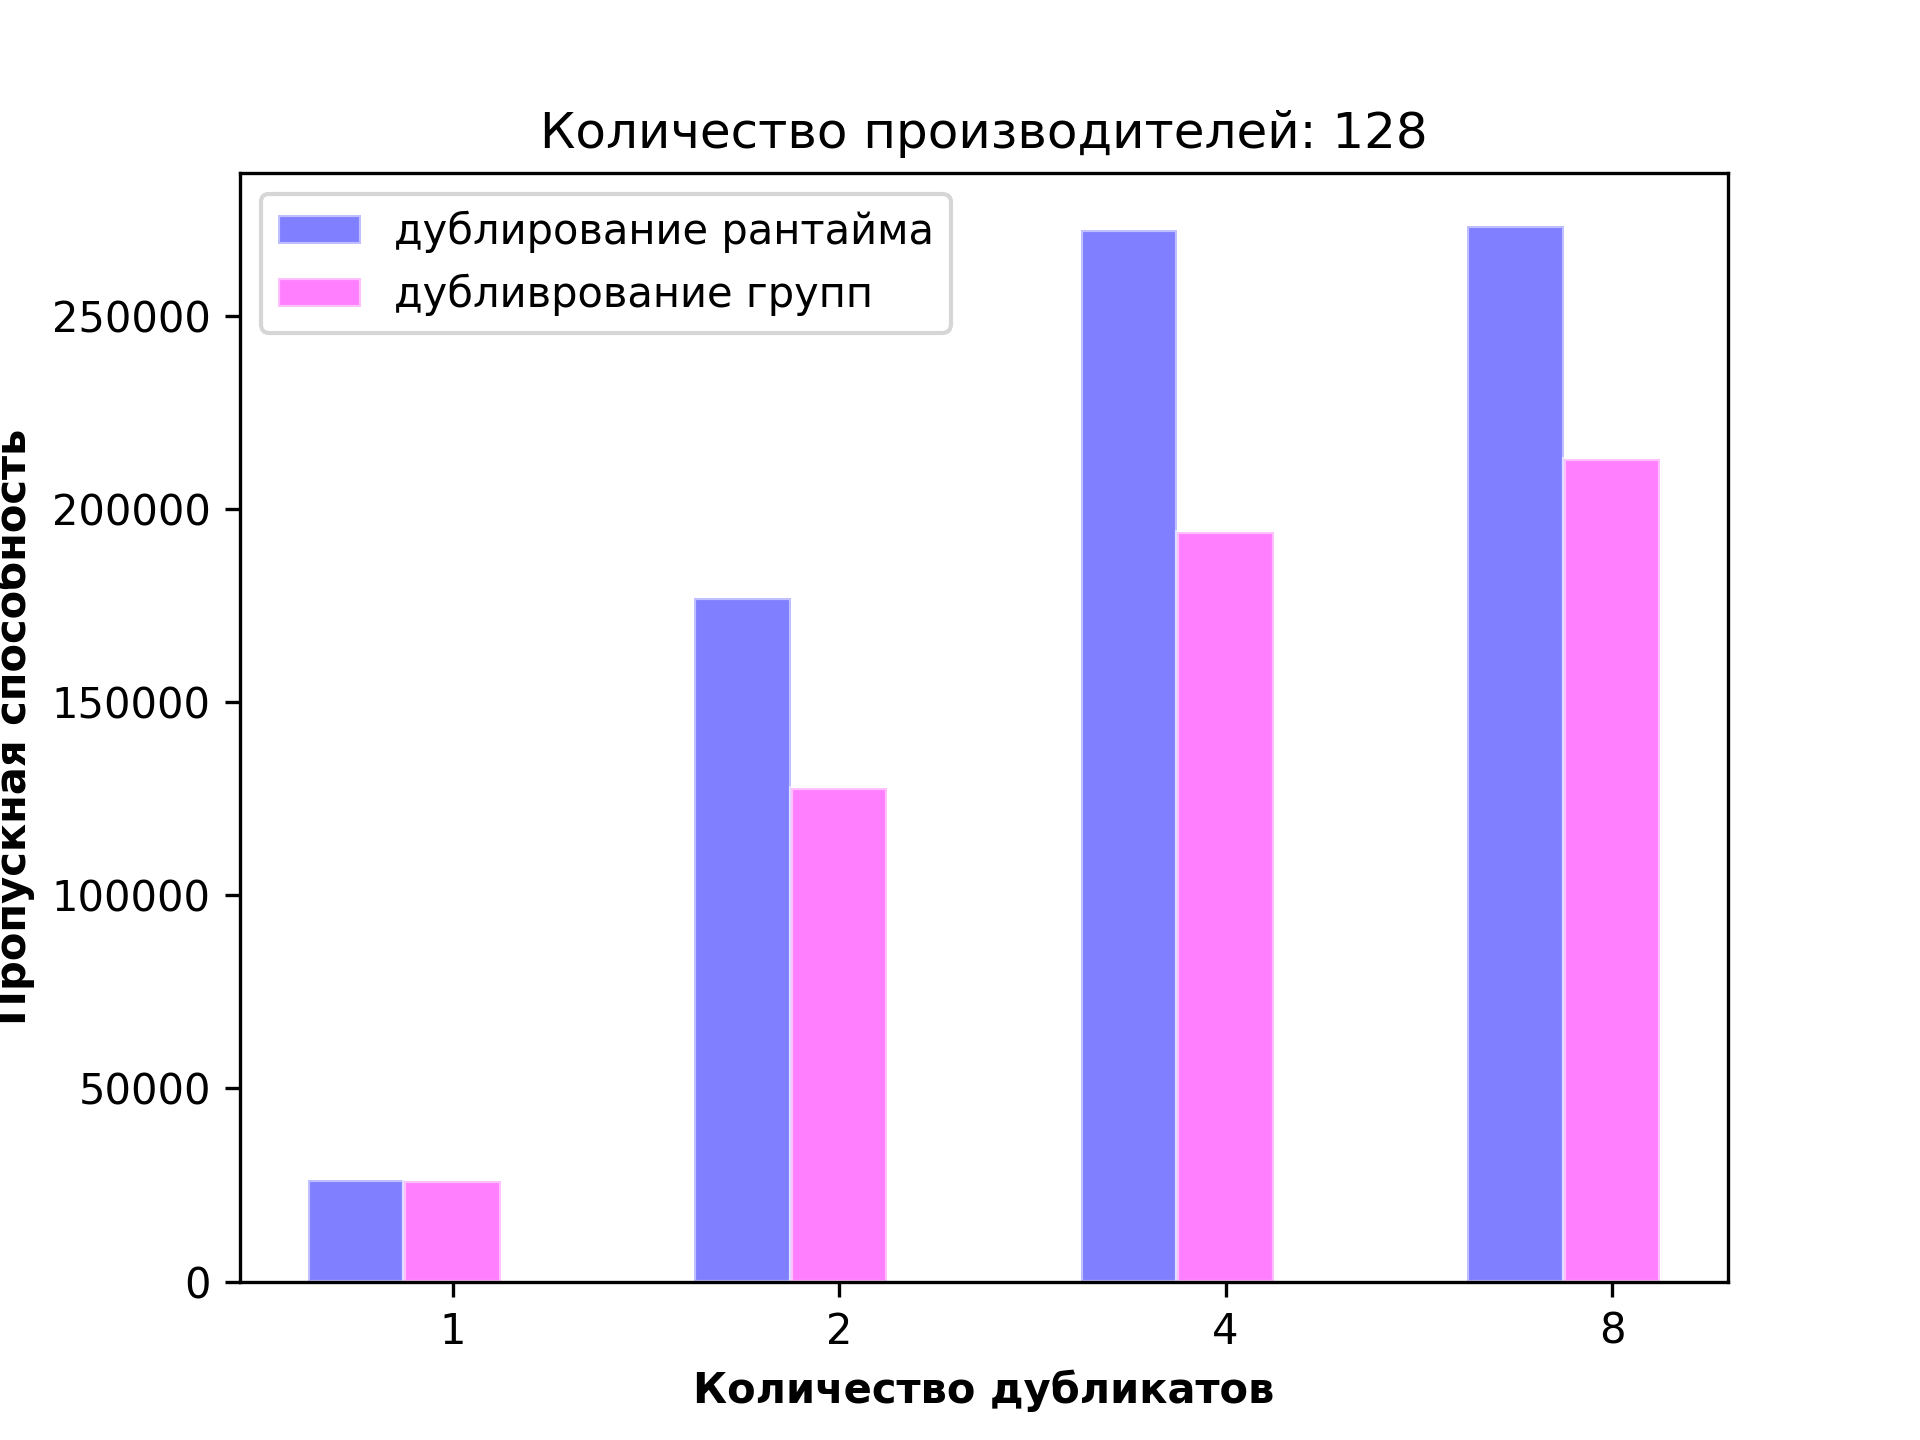
\includegraphics[scale=0.80]{pictures/rt_gp_128_1000.png}}
    \end{center}

    \caption{Производительность системы при использовании нескольких рантаймов}
    \label{fig:tatlin:multi_rt:eval}
\end{figure}

\subsection{Вывод}

% TODO(text)
